\chapter{研究の準備}\label{cha:Preparation}
本章では、本研究で必要となる前提知識を説明する。
% \section{モータ作成}\label{motor}
% \subsection{仕様書}\label{siyo}
% \subsection{シミュレータの役割}\label{simu}
\section{Modelica言語}\label{modelica}
微分代数方程式を用いた、複合領域の物理システムモデリングのために開発されたオブジェクト指向言語である。\\
 \subsection{Modelica標準ライブラリ(MSL)}\label{MSL}
        Modelica言語による様々な物理領域のモデルライブラリを開発しており、
        数学、機械、電気、熱、流体、制御系、状態遷移機械などを含んだフリーのライブラリがリリースされている。

\section{OpenModelica}\label{OM}
Modelica言語に対応したOSSである\cite{fritzson2006openmodelica}。
OpenModelicaから出力されるcsvファイルのファイル名は、「シミュレーションしたモデルの名前\_res.csv」で生成される。\\
仮に、シミュレーションしたモデルの名前が、「hoge」だった場合、csvファイルのファイル名は「hoge\_res.csv」となる。
\subsection{出力}\label{sub:output}
OpenModelicaでは、シミュレーション結果の保存先を、以下の3つの形式から選択することができる。
\begin{itemize}
    \item matファイル
    \item pltファイル
    \item csvファイル
\end{itemize}
今回試作するモータ特性表自動生成ツールでは、csvファイルにのみ対応する。\\
OpenModelicaから出力されるcsvファイルの一部を、図\ref{fig:simyu_csv}に示す。\\
csvファイルの1列目には、時間を表す「time」が必ず入る。\\
1行目には、「time」以外はオブジェクト名を含んだ変数名が必ず入る。\\

また、OpenModelicaでは、シミュレーション結果を、グラフとして画面上に描画することが可能である。
\begin{figure}[t]
	\centering
	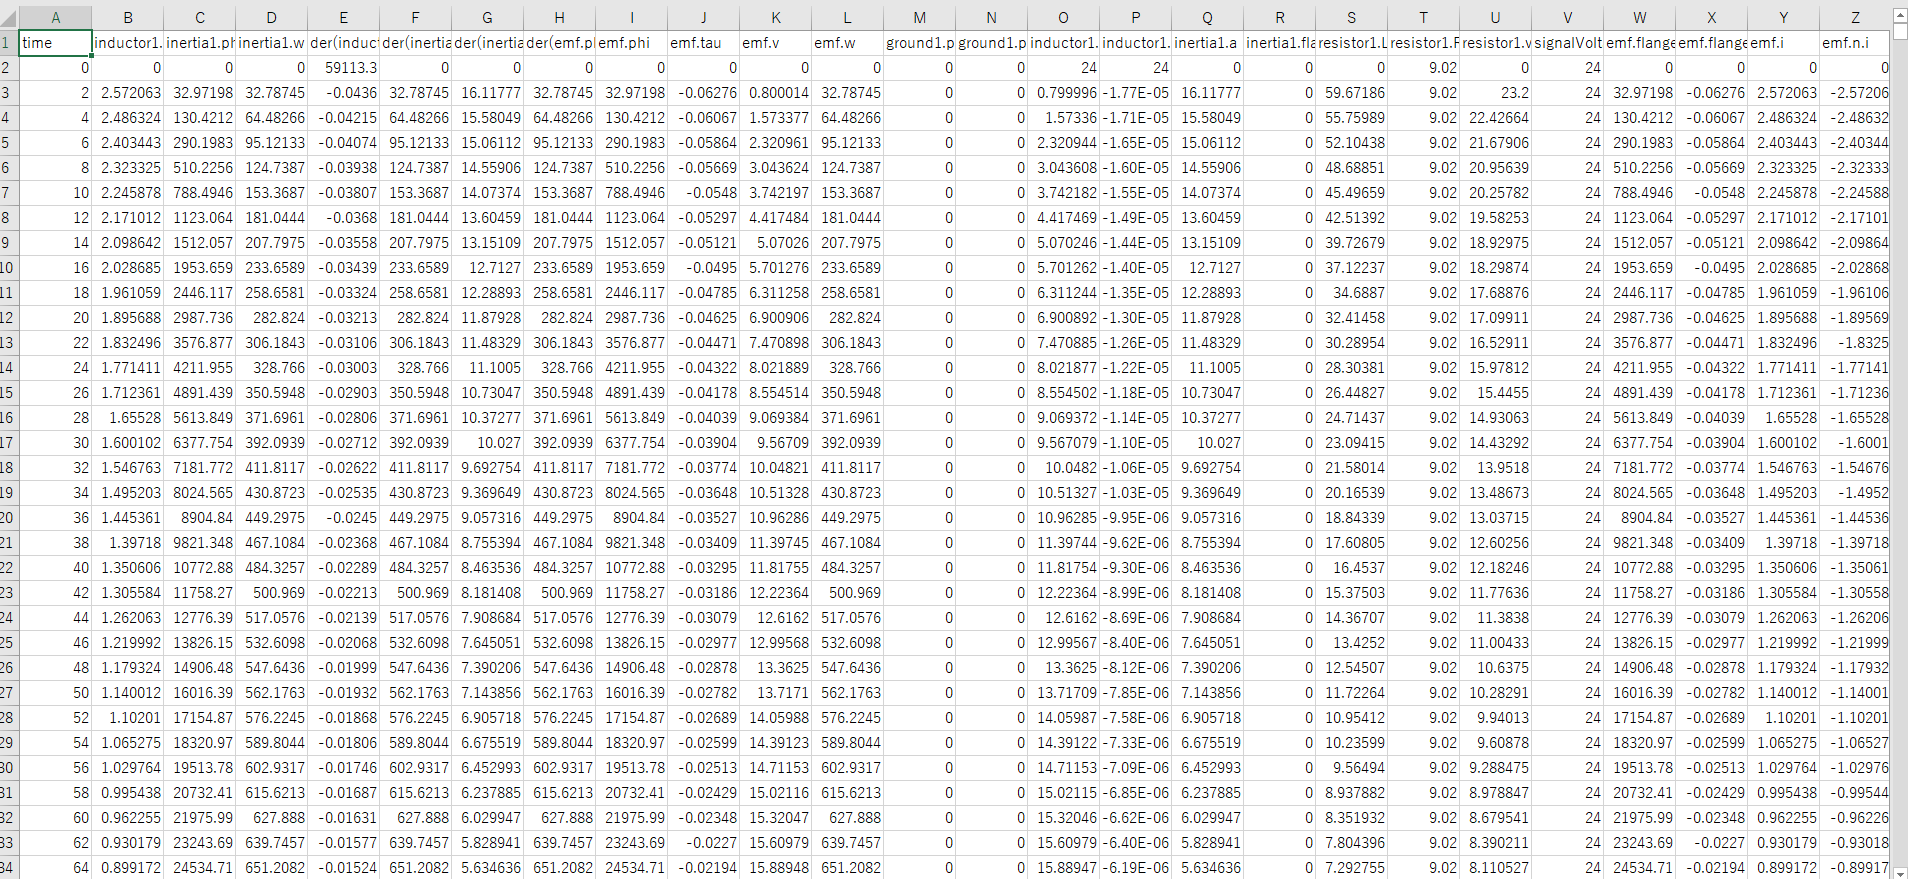
\includegraphics[width=16.5cm,height=10cm]{./Image/simyu_csv.png}
	\caption{シミュレーション結果のcsvファイルの一部}
	\label{fig:simyu_csv}
\end{figure}

\section{対応するモデル}\label{taioumodel}
試作するモータ特性表自動生成ツールでは、以下のModelicaモデルのシミュレーション結果に対応する。
\begin{itemize}
	\item ブラシ付きDCモータのModelicaモデル
	\item ブラシ付きDCモータのModelicaモデルをサブシステムとするモデル
\end{itemize}
以降、上記のモデルについて具体的に説明する。

\subsection{ブラシ付きDCモータのModelicaモデル}\label{sub:tanntai}
ブラシ付きDCモータのModelicaモデルとは、ブラシ付きDCモータの等価回路\cite{等価回路}をModelica言語で表したモデルのことである。\\
ブラシ付きDCモータの等価回路をModelica言語で表すためには、電源部品、抵抗部品、インダクター部品、起電力部品、慣性部品、接地部品が必要である。\\
% 上記6つの部品が必要な理由は、ブラシ付きDCモータの等価回路\cite{等価回路}をModelica言語で表す際に、使用する部品\cite{modelicaシステム本}だからである。\\
また、電源部品、抵抗部品、インダクター部品、起電力部品、慣性部品には、それぞれ以下のパラメータを設定しなければならない。
\begin{itemize}
	\item 電源部品 ・・・ 電圧値 V
	\item 抵抗部品 ・・・ 抵抗値 $\Omega$
	\item インダクター部品 ・・・ インダクタンス値 H
	\item 起電力部品 ・・・ トルク定数 N.m/A
	\item 慣性部品 ・・・ 慣性モーメント kg.m2
\end{itemize}
各部品で使用するMSLを表\ref{tab:MSL}に、ブラシ付きDCモータの等価回路を図\ref{fig:touka}に、ブラシ付きDCモータのModelicaモデルの例を図\ref{fig:tantai_model}に、
図\ref{fig:tantai_model}のModelicaコードを図\ref{fig:tantai_modelica}に、それぞれ示す。

\begin{table}[t]
	\centering
	\caption{MSL対応表}
	\begin{tabular}{|c|c|} \hline
	  部品名 & 使用するMSL \\ \hline \hline
	  電源部品 & Modelica.Electrical.Analog.Sources \\ \hline
	  抵抗部品 & Modelica.Electrical.Analog.Basic \\ \hline
	  インダクター部品 & Modelica.Electrical.Analog.Basic \\ \hline
	  起電力部品 & Modelica.Electrical.Analog.Basic \\ \hline
	  慣性部品 & Modelica.Mechanics.Rotational.Components \\ \hline
	  接地部品 & Modelica.Electrical.Analog.Basic \\ \hline
	\end{tabular}
	\label{tab:MSL}
  \end{table}
 
\begin{figure}[t]
	\centering
	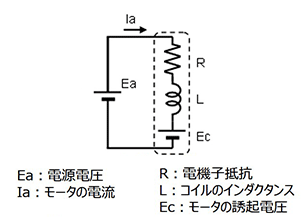
\includegraphics[width=7cm]{./Image/touka.png}
	\caption{ブラシ付きDCモータの等価回路}
	\label{fig:touka}
  \end{figure}

\begin{figure}[t]
  \centering
  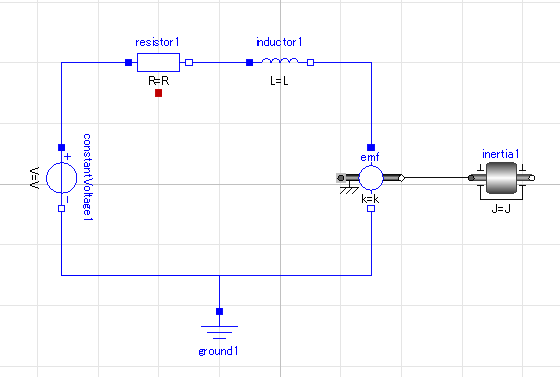
\includegraphics[width=10cm]{./Image/tantai_model.png}
  \caption{ブラシ付きDCモータのModelicaモデルの例}
  \label{fig:tantai_model}
\end{figure}


% \begin{figure*}[t]
% 	\lstinputlisting[label={code:motor}, caption={図\ref{fig:tantai_model}のModelicaコード}]{./chapters/motor.mo}
% \end{figure*}

\begin{figure}[t]
	\centering
	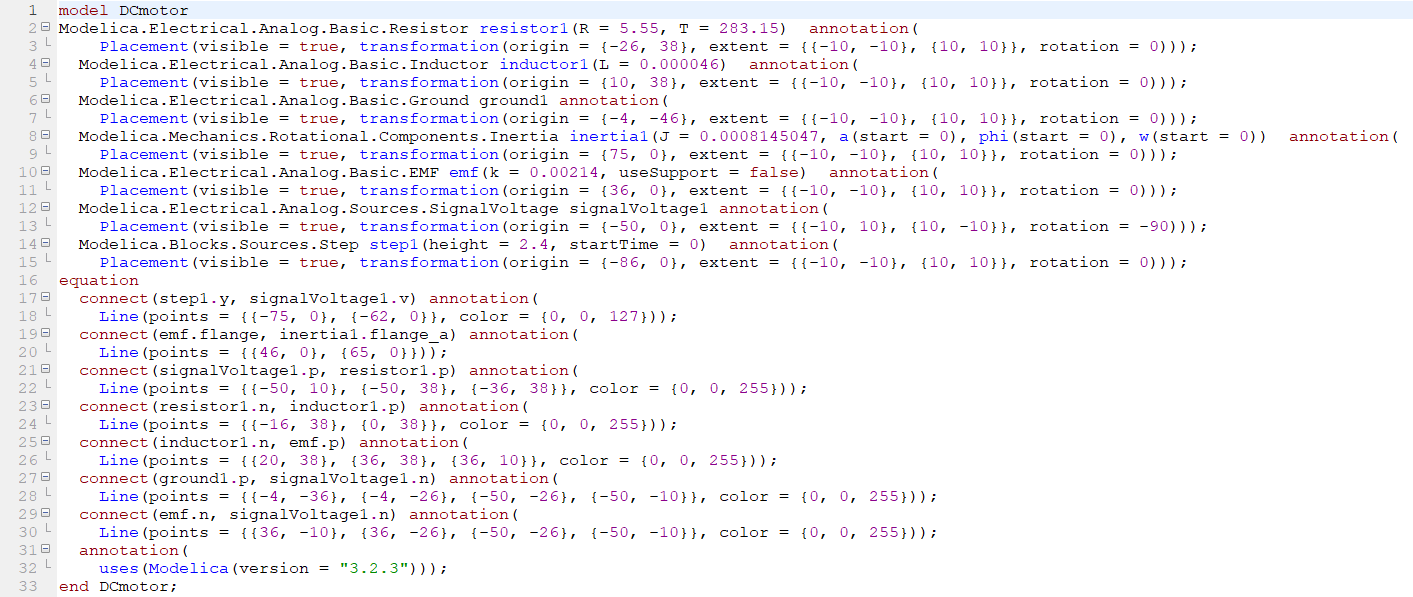
\includegraphics[width=16.5cm,height=8cm]{./Image/tantai_modelica.png}
	\caption{図\ref{fig:tantai_model}のModelicaコード}
	\label{fig:tantai_modelica}
  \end{figure}

%   \vspace{-1zh}

\subsection{ブラシ付きDCモータのModelicaモデルをサブシステムとするモデル} \label{sub:submodel}
ブラシ付きDCモータのModelicaモデルをサブシステム\cite{modelicaシステム本}とするモデルとは、
\ref{sub:tanntai}節で説明したブラシ付きDCモータのModelicaモデルを1つのサブシステムとして扱い、他の部品と合わせたモデルのことである。\\
例として、DCモータのサブシステムを用いたDCモータサーボのモデルを図\ref{fig:submodel}に、図\ref{fig:submodel}のModelicaコードを図\ref{fig:sub_modelica}に、それぞれ示す。

\begin{figure}[t]
	\centering
	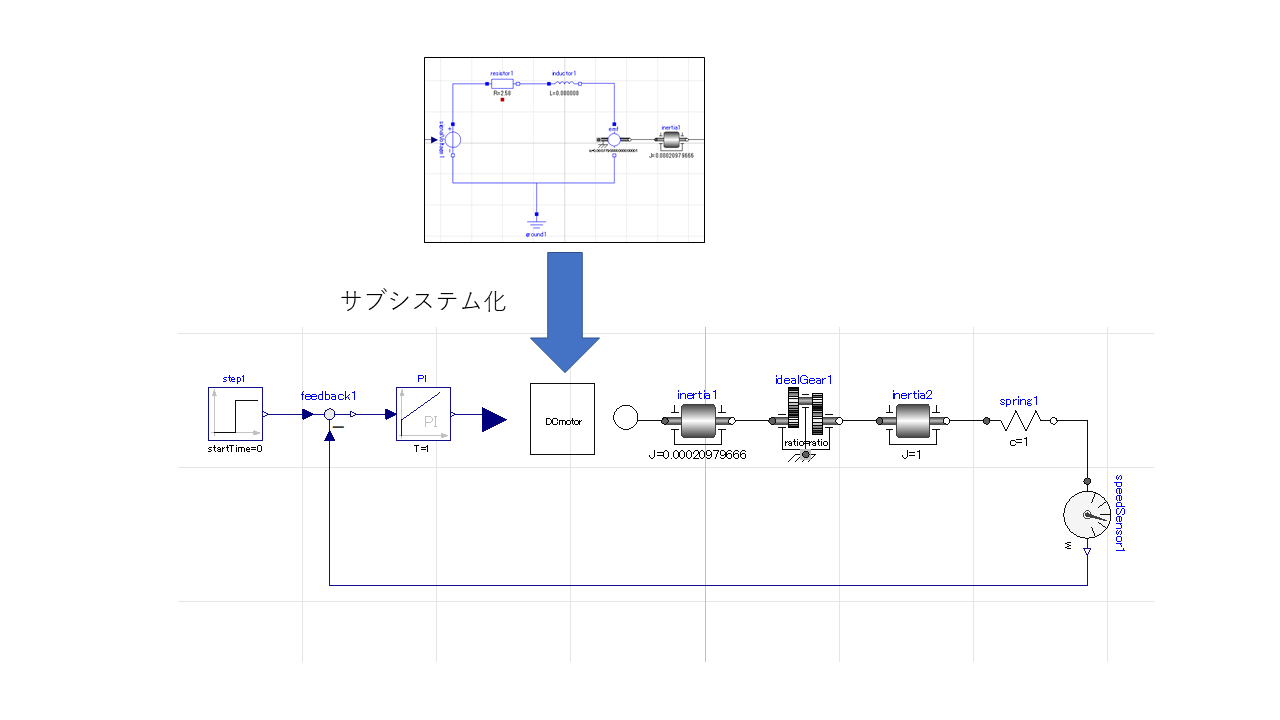
\includegraphics[width=16.5cm,height=10cm]{./Image/submodel_pack.png}
	\caption{DCモータサーボのモデル}
	\label{fig:submodel}
  \end{figure}

  \begin{figure}[t]
	\centering
	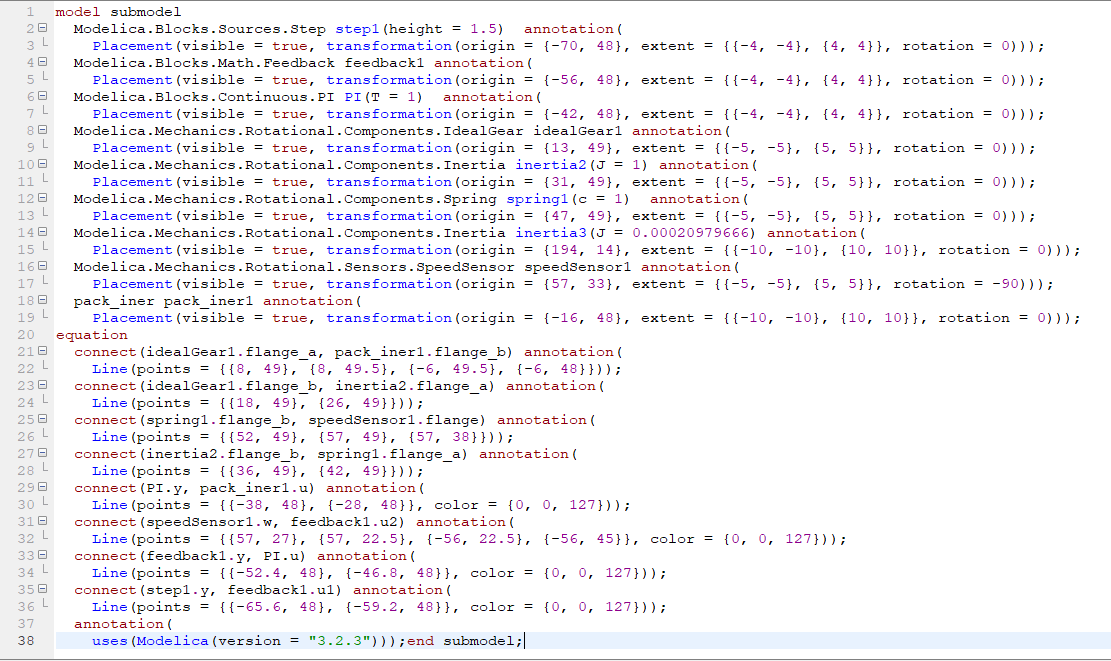
\includegraphics[width=16.5cm,height=10cm]{./Image/sub_modelica.png}
	\caption{図\ref{fig:submodel}のModelicaコード}
	\label{fig:sub_modelica}
  \end{figure}

  \subsection{モデル作成時の制約}\label{sub:seiyaku}
  \ref{sub:tanntai}章、\ref{sub:submodel}章で説明した制約の他に、以下の制約も満たしていなければならない。

  \begin{itemize}
	  \item 入力は0秒スタート
	  \item 電圧値は一定
	  \item 各部品に名前をつける際は、デフォルトの名前にする
	  \item モータのモデルは1つまで
  \end{itemize}


  \section{ブラシ付きDCモータ}\label{}
  % ブラシ付きDCモータだけかけばいいのか?モータ全体の話も必要か?
  ブラシ付きモータとは、ーーー 
  今回試作するツールでは、ブラシ付きモータのシミュレーション結果に対応する。
  
\section{モータ特性表}\label{mortoku}
モータ特性表とは、モータを選定する際に、参考にする資料である。一般的に決まった形式はなく、各会社によって書いている要素は異なるため、
10社のモータ特性表をもとに、作成するモータ特性表の要素を決定した。\\
以下にモータ特性表の構成と、要素を示す。

  \section{Python}\label{python}
  !!!未調査!!!
  使用するライブラリ?モジュール?をかく?
% Javaは、1990年代前半にSun MicrosystemsでJames Arthur Gosling、Wiliam Nelson Joyなどの人々が開発したプログラミング言語およびプラットフォームである。
% Javaはクラスベースのオブジェクト指向プログラミング言語である。
% Javaのプログラムは複数のクラスから構成され、クラス定義からそのクラスのインスタンスであるオブジェクトを何個でも作ることができる%\cite{プログラミング言語Java}。

% 1つのjavaファイルには複数のクラスを記述できる。
% 各クラスにはメンバが存在し、メンバの主な種類はフィールドとメソッドである。
% フィールドは、クラス自身あるいはそのクラスのオブジェクトのどちらかに属しているデータ変数である。
% メソッドは、クラスの状態を操作するためにフィールドに対して実行可能な処理を行う振舞いである。

% 今回実装すは、で開発する。